\section{Bestiaire}

\subsection{Rakghoul}
\label{sec:rakghoul}
\noindent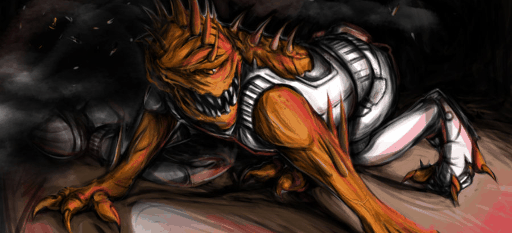
\includegraphics[width=\linewidth]{_img/bestiary/rakghoul.png}

\paragraph{Background}
Les Rakghouls sont une espèce issue d’une maladie créée par le seigneur Sith Karness Muur. Les individus atteint par cette maladie deviennent des monstres incapables de penser par eux-mêmes. Karness peut les contrôler grâce à son talisman (Le Talisman de Muur).

La maladie se transmet par une griffure ou une morsure mais cela ne fonctionne pas avec les êtres sensibles à la Force. Karness a créé ce virus à partir du coté Obscur de la Force ce qui explique une forte présence obscure près de ces monstres.

Karness a créé plusieurs versions du virus car les premiers Rakghouls ne répondaient pas bien au contrôle de Karness. Les nouveaux sont plus réceptifs et plus fort.

Quand le Talisman de Muur a été perdu dans les bas fonds de Taris, on a peu constaté que les créatures, suite à une exposition prologée au Talisman finissaient par se transformer en Rakghouls. Mais les Rakghouls transformé de cette façon sont bestiaux, stupides et sans âme. Ils attaquent tout ce qui bouge. Ces créatures ne fonctionnent qu’à l’instinct.

\paragraph{Traits}

\begin{itemtable}[ c c c c c ]
    \textbf{Agi} & \textbf{Int} & \textbf{\^Ame} & \textbf{For} & \textbf{Vig} \\
    d8           & d6           & d6             & d8           & d8
\end{itemtable}
\begin{itemtable}[ l X ]
    \textbf{Allure}      & 6 \\
    ~                    & Vision Nocturne \\
    ~                    & Marche sur les murs \\
    \textbf{Compétences} & Combat d8, Discrétion d6
\end{itemtable}

\paragraph{Attaque / Défense}
\begin{itemtable}[ c c ]
    \textbf{Parade}     & \textbf{Résistance} \\
    6                   & 6 
\end{itemtable}

\begin{itemtable}[ X c c ]
    ~       & \textbf{Combat}   & \textbf{Dégats} \\
    Griffes & d8                & 1d6 
\end{itemtable}

\newpage
\subsection{Rakghoul Amblyope}
\label{sec:rakghoul-amblyope}
\noindent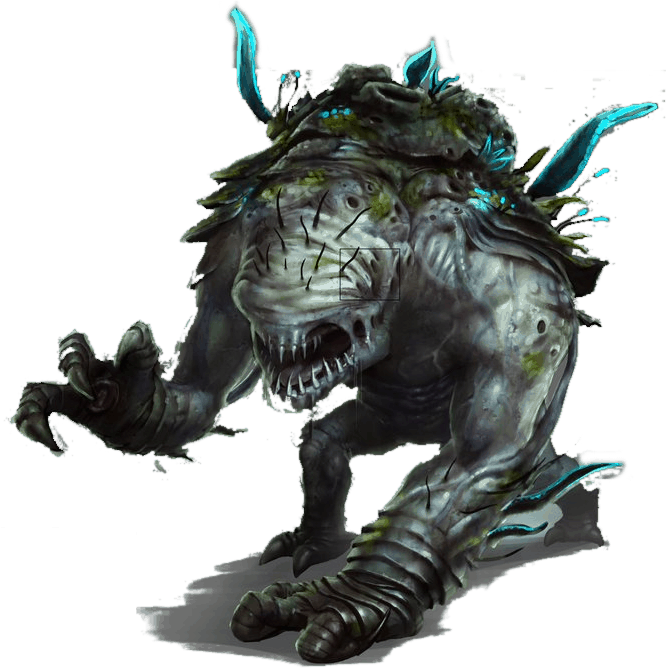
\includegraphics[height=200pt]{_img/bestiary/rakghoul-amblyope.png}

\paragraph{Background}
Version stéroïdée des Rakghouls standard, Amblyope est notre petit boss de niveau.

Quand les Rakghouls sont livrés à eux-mêmes et qu’ils laissent libre cours à leurs plus bas instincts, il arrive qu’un Rakghoul plus fort que les autres s’en prenne à ces petits camarades et les dévore sans scrupules. Cet afflux de Force Obscure peut le faire muter et le Rakghoul devient une espèce de gros monstre de 3m de haut, complètement aveugle mais attiré par les émanations de Force, il attaque machinalement les adversaires les plus sensibles à la Force. 

\paragraph{Traits}

\begin{itemtable}[ c c c c c ]
    \textbf{Agi} & \textbf{Int} & \textbf{\^Ame} & \textbf{For} & \textbf{Vig} \\
    d4           & d6           & d6             & d12+2        & d10
\end{itemtable}
\begin{itemtable}[ l X ]
    \textbf{Allure}      & 5 \\
    \textbf{Taille}      & +5 \\
    ~                    & Vision de Force \\
    ~                    & \'Enorme (+2 pour les jets d’attaque adverses)\\
    \textbf{Compétences} & Combat d10
\end{itemtable}

\paragraph{Défense / Attaque}
\begin{itemtable}[ c c ]
    \textbf{Parade}     & \textbf{Résistance} \\
    5                   & 12 
\end{itemtable}

\begin{itemtable}[ X c c ]
    ~           & \textbf{Combat}   & \textbf{Dégats} \\
    Mains nues  & d10               & d12+2 
\end{itemtable}

\clearpage

\subsection{Contrebandier (Taris)} \label{sec:taris-contrebandier}
\begin{figure}[h!]
    \centering
    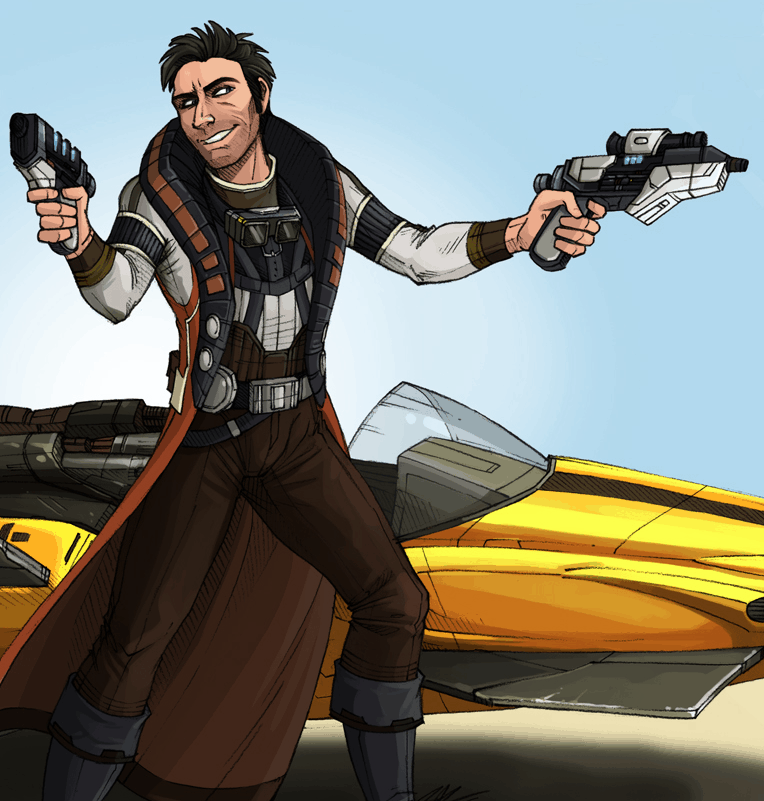
\includegraphics[height=200pt]{_img/bestiary/contrebandier.png}
\end{figure}
\paragraph{Background}
Les bas-fonds de Taris grouillent de toutes sortes de malfrats. C’est un des coins favoris de contrebandiers qui peuvent y kidnapper de jeunes enfants en toute impunité. Personne ne viendra se plaindre de la disparition d’une vermine de plus dans les bas fond.

Ce ne sont en général que des débutants attiré par la facilité. Seul ils ne représentent pas un grand danger, mais ils se promènent souvent en groupe.

\paragraph{Traits}

\begin{itemtable}[ c c c c c ]
    \textbf{Agi} & \textbf{Int} & \textbf{\^Ame} & \textbf{For} & \textbf{Vig} \\
    d6           & d6           & d4             & d8           & d8
\end{itemtable}
\begin{itemtable}[ l X ]
    \textbf{Allure}      & 6 \\
    \textbf{Compétences} & Combat d8, Tir d10
\end{itemtable}

\paragraph{Défense}
\begin{itemtable}[ c c ]
    \textbf{Parade}     & \textbf{Résistance} \\
    5                   & 6 (+1)
\end{itemtable}

\paragraph{Attaque}
\begin{itemtable}[ X c c ]
    ~           & \textbf{Combat}   & \textbf{Dégats} \\
    Blaster     & -                 & 2d6+1
\end{itemtable}


\newpage

\subsection{Storm Trooper} \label{sec:storm-trooper}
\begin{figure}[h!]
    \centering
    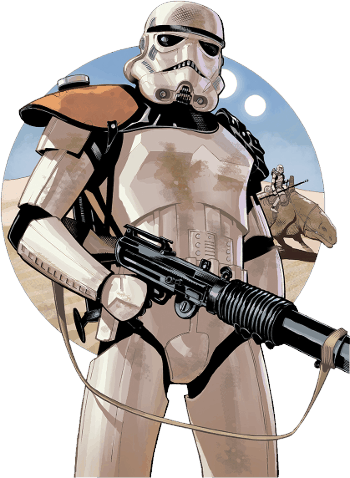
\includegraphics[height=200pt]{_img/bestiary/stormtrooper.png}
\end{figure}
\paragraph{Background}
Soldats dévoué de l’empire. Certain sont des clones restant de la guerre des clones d’autres non. Ils sont entrainés au combat, équipé d’une bonne armure et armé de Fusil Blaster efficaces.

\paragraph{Traits}

\begin{itemtable}[ c c c c c ]
    \textbf{Agi} & \textbf{Int} & \textbf{\^Ame} & \textbf{For} & \textbf{Vig} \\
    d4           & d6           & d4             & d8           & d8
\end{itemtable}
\begin{itemtable}[ l X ]
    \textbf{Allure}      & 6 \\
    \textbf{Compétences} & Combat d10, Tir d10
\end{itemtable}

\paragraph{Défense}
\begin{itemtable}[ c c ]
    \textbf{Parade}     & \textbf{Résistance} \\
    7                   & 6 (+4)
\end{itemtable}

\paragraph{Attaque}
\begin{itemtable}[ X c c ]
    ~              & \textbf{Combat}   & \textbf{Dégats} \\
    Fusil Blaster  & -                 & 2d8 (3)
\end{itemtable}


\newpage
\subsection{Wampa} \label{sec:wampa}
\begin{figure}[h!]
    \centering
    
\includegraphics[height=200pt]{_img/bestiary/wampa.png}
\end{figure}

\paragraph{Background}
Créature capable de supporter les plus froides températures, le Wampa est un féroce prédateur agissant surtout la nuit. Bien que sa planète d’origine soit Hoth, on retrouve des Wampas sur quelques autres mondes, mais leur férocité les rend difficiles à exporter, et on trouve peu de candidats assez fous pour tenter l’expérience. 

\paragraph{Traits}

\begin{itemtable}[ c c c c c ]
    \textbf{Agi} & \textbf{Int} & \textbf{\^Ame} & \textbf{For} & \textbf{Vig} \\
    d8           & d6           & d6             & d8           & d8
\end{itemtable}
\begin{itemtable}[ l X ]
    \textbf{Allure}      & 6 \\
    ~                    & Vision Nocturne \\
    ~                    & Marche sur les murs \\
    \textbf{Compétences} & Combat d8, Discrétion d6
\end{itemtable}

\paragraph{Attaque / Défense}
\begin{itemtable}[ c c ]
    \textbf{Parade}     & \textbf{Résistance} \\
    6                   & 6 
\end{itemtable}

\begin{itemtable}[ X c c ]
    ~       & \textbf{Combat}   & \textbf{Dégats} \\
    Griffes & d8                & 1d6 
\end{itemtable}

\newpage

\subsection{Cybercleps} \label{sec:cybercleps}
\begin{figure}[h!]
    \centering
    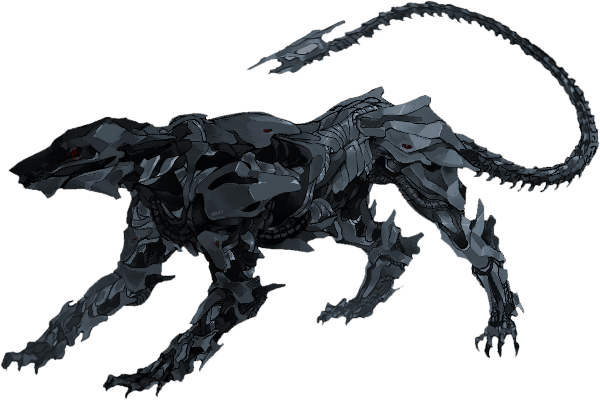
\includegraphics[width=\linewidth]{_img/bestiary/cybercleps.png}
\end{figure}
\paragraph{Background}
Les Cybercleps sont des créatures artificielles conçues pour tenir éloigné les curieux de certaines zones. Ce sont des drônes capable d’une complète autonomie mais leur efficacité est bien meilleure quand elles sont contrôllé par une IA centrale. 

Adaptées au gardiennage de batiments de à la sécurité des villas, leur conception ne les prédestine pas à devenir des animaux de compagnie, même avec la programmation adéquate !

Lorsqu’ils sont commandé par un central, leur programmation les rend particulièrement efficace. Ils deviennent capable d’attaquer en groupe et de se concentrer sur les proies plus faible. Ils sont capable de stratégies de combat pour venir à bout de groupe plus nombreux qu’eux.

Les Cybercleps restent combatif même blessé grièvement, tant que le processeur principal présent dans leur tête n’est pas détruit.
\paragraph{Traits}

\begin{itemtable}[ c c c c c ]
    \textbf{Agi} & \textbf{Int} & \textbf{\^Ame} & \textbf{For} & \textbf{Vig} \\
    d8           & d4           & d4             & d8           & d8
\end{itemtable}
\begin{itemtable}[ l X ]
    \textbf{Allure}      & 7 \\
    \textbf{Compétences} & Combat d10 \\
    \textbf{Atouts}      & Grande esquive \par Créature artificielle
\end{itemtable}

\paragraph{Défense / Attaque}
\begin{itemtable}[ c c ]
    \textbf{Parade}     & \textbf{Résistance} \\
    8                   & 6
\end{itemtable}

\begin{itemtable}[ X c c ]
    ~              & \textbf{Combat}   & \textbf{Dégats} \\
    Griffe         & -                 & 1d8 (2)         \\
    Crocs          & -                 & 2d6 (1)
\end{itemtable}

\subsection{Corvette de l’Empire} \label{sec:empire-corvette}

\subsection{Chasseur TIE} \label{sec:tie-fighter}